\documentclass[12pt,a4paper]{report}
\usepackage[utf8]{inputenc}
\usepackage[french]{babel}
\usepackage[T1]{fontenc}
\usepackage{lmodern}
\usepackage{graphicx}
\usepackage{geometry}
\usepackage{fancyhdr}
\usepackage{titlesec}
\usepackage{hyperref}
\usepackage{listings}
\usepackage{xcolor}
\usepackage{float}
\usepackage{amsmath}
\usepackage{enumitem}
\usepackage{tikz}
\usepackage{pgfplots}
\usepackage{booktabs}
\usepackage{array}
\usepackage{tcolorbox}
\usepackage{amssymb}

% Configuration de la page
\geometry{
    left=2.5cm,
    right=2.5cm,
    top=2.5cm,
    bottom=2.5cm
}

% ============= COLORS =============
\definecolor{maincolor}{RGB}{30,58,138}       % Bleu ENSA (primary blue)
\definecolor{secondcolor}{RGB}{249,115,22}    % Orange ENSA (accent orange)
\definecolor{graytext}{RGB}{80,80,80}
\definecolor{lightgray}{RGB}{240,240,240}
\definecolor{codegreen}{RGB}{0,128,0}
\definecolor{codegray}{RGB}{128,128,128}
\definecolor{codepurple}{RGB}{153,0,153}
\definecolor{backcolour}{RGB}{248,248,248}
\definecolor{bleuENSA}{RGB}{30,58,138}        % Reprend maincolor
\definecolor{orangeENSA}{RGB}{249,115,22}     % Reprend secondcolor
\definecolor{jauneENSA}{RGB}{255,202,40}
\definecolor{grisclairENSA}{RGB}{215,215,215}
\definecolor{grisENSA}{RGB}{120,120,120}

% Configuration des hyperliens
\hypersetup{
    colorlinks=true,
    linkcolor=maincolor,
    filecolor=maincolor,
    urlcolor=secondcolor,
    citecolor=maincolor,
    pdftitle={Rapport de Projet - Application de Gestion Pédagogique},
    pdfauthor={Équipe ENSA Tétouan},
    pdfsubject={Application Android de Gestion Pédagogique},
    pdfkeywords={Android, Gestion Pédagogique, ENSA, Mobile}
}

% Configuration des listings
\lstdefinestyle{javastyle}{
    backgroundcolor=\color{backcolour},
    commentstyle=\color{codegreen},
    keywordstyle=\color{maincolor}\bfseries,
    numberstyle=\tiny\color{codegray},
    stringstyle=\color{codepurple},
    basicstyle=\ttfamily\small,
    breakatwhitespace=false,
    breaklines=true,
    captionpos=b,
    keepspaces=true,
    numbers=left,
    numbersep=5pt,
    showspaces=false,
    showstringspaces=false,
    showtabs=false,
    tabsize=4,
    frame=single,
    rulecolor=\color{lightgray}
}
\lstset{style=javastyle}

% Configuration des en-têtes et pieds de page
\pagestyle{fancy}
\fancyhf{}
\fancyhead[L]{\small\textcolor{graytext}{\leftmark}}
\fancyhead[R]{\small\textcolor{graytext}{\thepage}}
\fancyfoot[C]{\thepage}
\renewcommand{\headrulewidth}{0.4pt}
\renewcommand{\footrulewidth}{0.4pt}

% Configuration des titres
\titleformat{\chapter}[display]
{\normalfont\huge\bfseries\color{maincolor}}{\chaptertitlename\ \thechapter}{20pt}{\Huge}

\titleformat{\section}
    {\normalfont\Large\bfseries\color{maincolor}}
    {\thesection}{1em}{}[\titlerule]

\titleformat{\subsection}
    {\normalfont\large\bfseries\color{maincolor}}
    {\thesubsection}{1em}{}

\titleformat{\subsubsection}
    {\normalfont\normalsize\bfseries\color{secondcolor}}
    {\thesubsubsection}{1em}{}

% ============= CUSTOM BOXES =============
\newtcolorbox{infobox}[1][]{
    colback=secondcolor!5!white,
    colframe=secondcolor,
    fonttitle=\bfseries,
    title=#1,
    arc=2mm
}

\newtcolorbox{warningbox}[1][]{
    colback=jauneENSA!10!white,
    colframe=jauneENSA!80!black,
    fonttitle=\bfseries,
    title=#1,
    arc=2mm
}

\newtcolorbox{successbox}[1][]{
    colback=green!5!white,
    colframe=green!70!black,
    fonttitle=\bfseries,
    title=#1,
    arc=2mm
}

% ============================================
% DÉBUT DU DOCUMENT
% ============================================

\begin{document}

% Page de garde
\begin{titlepage}
    % Fond graphique avec bandes colorées
    \begin{tikzpicture}[remember picture,overlay]
        % Bandes latérales
        \fill[bleuENSA!95!black] (current page.north west) rectangle
            ([xshift=1.8cm]current page.south west);
        \fill[orangeENSA!80!black] (current page.north east) rectangle
            ([xshift=-1.4cm]current page.south east);

        % Liseré accentué à gauche
        \fill[jauneENSA] ([xshift=1.5cm]current page.north west) rectangle
            ([xshift=1.65cm]current page.south west);

        % Bandes diagonales fines et parallèles (droite)
        \begin{scope}[shift={(current page.south east)},rotate=66]
            \fill[grisclairENSA] (0,0) rectangle (0.35cm,15cm);
        \end{scope}
        \begin{scope}[shift={(current page.south east)},rotate=66]
            \fill[orangeENSA] (-0.8cm,0.2cm) rectangle (-0.45cm,15.2cm);
        \end{scope}
        \begin{scope}[shift={(current page.south east)},rotate=66]
            \fill[jauneENSA] (-1.6cm,0.4cm) rectangle (-1.25cm,15.4cm);
        \end{scope}
    \end{tikzpicture}

    {\sffamily
    % Logo ENSA petit en haut à droite
    \begin{flushright}
        \vspace*{-1cm}
        \hspace*{-2cm}
        \includegraphics[width=0.12\textwidth]{conception-diagrams/ENSA_logo.png} % PLACEHOLDER: Logo ENSA
    \end{flushright}
    
    % Espacement avant le titre
    \vspace*{1.0cm}

    % École
    \noindent
    {\Large\bfseries\color{bleuENSA!80!black}\MakeUppercase{École Nationale des Sciences Appliquées}}\\[0.2cm]
    {\large\bfseries\color{bleuENSA!80!black}de Tétouan}\\[0.7cm]
    
    % Titre principal
    {\fontsize{28}{34}\selectfont\bfseries Application de Gestion \\[0.1cm] Pédagogique \\[0.1cm] pour ENSA Tétouan}\\[0.6cm]
    
    {\normalsize\itshape\color{grisENSA}Application Android pour la digitalisation\\[0.1cm]
    de la gestion pédagogique de l'école}

    \vspace{1.5cm}

    % Section Équipe
    \begin{flushright}
        {\large\bfseries\color{bleuENSA!80!black}Équipe de Développement:}\\[0.3cm]
        \begin{tabular}{r@{\hspace{0.4cm}}l}
            \textbf{RAISSOUNI} & Abdellah (Chef de Projet) \\[0.1cm]
            \textbf{BENCAID} & Mouad \\[0.1cm]
            \textbf{LARAICHI} & Yassine \\[0.1cm]
            \textbf{ELKHOUMSI} & Imane \\[0.1cm]
            \textbf{ABOULKACEM} & Asmae \\
        \end{tabular}
    \end{flushright}

    \vspace{1.0cm}

    % Section Encadrant et infos combinées
    \begin{flushright}
        {\large\bfseries\color{bleuENSA!80!black}Encadré par:}\\[0.2cm]
        {\large\bfseries Pr. Abdeljabbar MANSOUR}\\[0.6cm]
        
        {\normalsize\bfseries Année universitaire : 2024/2025}\\[0.2cm]
        {\normalsize\bfseries Filière : Génie Informatique}
    \end{flushright}

    \vspace*{0.5cm}
    }% fin style sans empattement
\end{titlepage}

% Page de remerciements
\newpage
\thispagestyle{empty}
\vspace*{5cm}
\begin{center}
    {\huge\bfseries Remerciements}
\end{center}

\vspace{2cm}

\begin{quotation}
    Nous tenons à exprimer notre profonde gratitude à tous ceux qui ont contribué de près ou de loin à la réalisation de ce projet.
    
    \vspace{1cm}
    
    Nos sincères remerciements vont en premier lieu à notre encadrant, \textbf{Pr. Abdeljabbar MANSOUR}, pour son encadrement, ses conseils précieux et sa disponibilité tout au long de ce projet.
    
    \vspace{0.5cm}
    
    Nous remercions également l'administration de l'École Nationale des Sciences Appliquées de Tétouan pour nous avoir fourni l'environnement et les ressources nécessaires à la réalisation de ce travail.
    
    \vspace{0.5cm}
    
    Enfin, nous remercions tous les membres de l'équipe pour leur collaboration, leur dévouement et leur esprit d'équipe qui ont rendu possible la réalisation de ce projet.
\end{quotation}

\newpage
\thispagestyle{empty}
\mbox{}

% Table des matières
\tableofcontents
\newpage
\listoffigures
\newpage
\listoftables

% ============================================
% CHAPITRES
% ============================================

\chapter{Introduction}
\thispagestyle{fancy}

\section{Contexte et Motivation}

L'École Nationale des Sciences Appliquées (ENSA) de Tétouan est un établissement d'enseignement supérieur qui forme des ingénieurs dans plusieurs spécialités. La gestion pédagogique de l'école implique de nombreuses tâches administratives et organisationnelles qui nécessitent une coordination efficace entre différents acteurs : le directeur adjoint, les professeurs assistants et les professeurs vacataires.

Actuellement, la gestion des formations, des emplois du temps, des réunions pédagogiques et des cahiers de charges se fait principalement de manière traditionnelle, ce qui peut entraîner des difficultés de coordination, des pertes de temps et des risques d'erreurs.

\section{Problématique}

La gestion pédagogique actuelle de l'ENSA Tétouan présente plusieurs défis :

\begin{itemize}
    \item \textbf{Manque de centralisation} : Les informations sont dispersées et difficiles à consulter
    \item \textbf{Communication inefficace} : Les échanges entre les différents acteurs sont souvent asynchrones
    \item \textbf{Gestion manuelle des emplois du temps} : Risque de conflits et de chevauchements
    \item \textbf{Suivi difficile des cahiers de charges} : Difficulté à suivre l'état d'avancement des validations
    \item \textbf{Planification des réunions complexe} : Coordination difficile des disponibilités
\end{itemize}

\section{Objectifs du Projet}

L'objectif principal de ce projet est de développer une application mobile Android permettant de digitaliser et d'optimiser la gestion pédagogique de l'ENSA Tétouan. Les objectifs spécifiques sont :

\begin{enumerate}
    \item Développer une application mobile intuitive et facile à utiliser
    \item Centraliser toutes les informations pédagogiques dans une base de données
    \item Faciliter la communication entre les différents acteurs
    \item Automatiser la gestion des emplois du temps
    \item Simplifier le processus de validation des cahiers de charges
    \item Améliorer la planification et le suivi des réunions pédagogiques
\end{enumerate}

\section{Structure du Rapport}

Ce rapport est organisé en plusieurs chapitres :

\begin{itemize}
    \item \textbf{Chapitre 1} : Introduction et contexte du projet
    \item \textbf{Chapitre 2} : Analyse et spécifications fonctionnelles
    \item \textbf{Chapitre 3} : Conception et architecture
    \item \textbf{Chapitre 4} : Implémentation et développement
    \item \textbf{Chapitre 5} : Tests et validation
    \item \textbf{Chapitre 6} : Conclusion et perspectives
\end{itemize}

\chapter{Analyse et Spécifications Fonctionnelles}

\section{Analyse des Besoins}

\subsection{Acteurs du Système}

L'application doit gérer trois types d'utilisateurs avec des rôles et permissions différents :

\subsubsection{Directeur Adjoint (Admin)}
Le Directeur Adjoint dispose de tous les droits d'administration sur le système :
\begin{itemize}
    \item Consulter tous les emplois du temps
    \item Élaborer et modifier les emplois du temps
    \item Planifier et gérer les réunions pédagogiques
    \item Approuver ou refuser les cahiers de charges
    \item Gérer les formations et modules
\end{itemize}

\subsubsection{Professeur Assistant}
Le Professeur Assistant dispose de droits limités :
\begin{itemize}
    \item Consulter son propre emploi du temps
    \item Créer et envoyer des cahiers de charges au directeur adjoint
    \item Consulter le planning des réunions auxquelles il participe
\end{itemize}

\subsubsection{Professeur Vacataire}
Le Professeur Vacataire dispose uniquement de droits de consultation :
\begin{itemize}
    \item Consulter son propre emploi du temps
    \item Consulter les réunions auxquelles il est invité
\end{itemize}

\section{Spécifications Fonctionnelles}

\subsection{Fonctionnalité 1 : Authentification}

L'application doit permettre aux utilisateurs de se connecter avec leurs identifiants (nom d'utilisateur et mot de passe). Le système doit :
\begin{itemize}
    \item Vérifier les identifiants dans la base de données
    \item Rediriger l'utilisateur vers le tableau de bord approprié selon son type
    \item Offrir une option "Se souvenir de moi" pour faciliter les connexions futures
\end{itemize}

% PLACEHOLDER: Screenshot de l'écran de connexion
\begin{figure}[H]
    \centering
    \includegraphics[width=0.4\textwidth]{screenshots/login-screen.png}
    \caption{Écran de connexion de l'application}
    \label{fig:login-screen}
\end{figure}

\subsection{Fonctionnalité 2 : Gestion des Formations}

Cette fonctionnalité permet au Directeur Adjoint de :
\begin{itemize}
    \item Consulter la liste des formations (initiale et continue)
    \item Créer de nouvelles formations
    \item Modifier les formations existantes
    \item Gérer les modules associés à chaque formation
    \item Valider ou refuser les formations en attente
\end{itemize}

% PLACEHOLDER: Screenshot de la gestion des formations
\begin{figure}[H]
    \centering
    \includegraphics[width=0.4\textwidth]{screenshots/formations-screen.png}
    \caption{Interface de gestion des formations}
    \label{fig:formations-screen}
\end{figure}

\subsection{Fonctionnalité 3 : Gestion des Réunions}

Cette fonctionnalité permet au Directeur Adjoint de :
\begin{itemize}
    \item Planifier de nouvelles réunions pédagogiques
    \item Sélectionner les participants parmi les utilisateurs
    \item Définir la date, l'heure et l'ordre du jour
    \item Modifier les réunions existantes
    \item Consulter l'historique des réunions
\end{itemize}

Les autres utilisateurs peuvent consulter les réunions auxquelles ils participent.

% PLACEHOLDER: Screenshot de la gestion des réunions
\begin{figure}[H]
    \centering
    \includegraphics[width=0.4\textwidth]{screenshots/reunions-screen.png}
    \caption{Interface de planification des réunions}
    \label{fig:reunions-screen}
\end{figure}

\subsection{Fonctionnalité 4 : Gestion des Cahiers de Charges}

Cette fonctionnalité permet :
\begin{itemize}
    \item \textbf{Pour le Professeur Assistant} :
    \begin{itemize}
        \item Créer un nouveau cahier de charges
        \item Télécharger un fichier (PDF, image, document)
        \item Modifier un cahier en brouillon
        \item Envoyer le cahier au Directeur Adjoint pour validation
    \end{itemize}
    \item \textbf{Pour le Directeur Adjoint} :
    \begin{itemize}
        \item Consulter tous les cahiers de charges
        \item Approuver ou refuser les cahiers envoyés
        \item Suivre l'état d'avancement des validations
    \end{itemize}
\end{itemize}

% PLACEHOLDER: Screenshot de la gestion des cahiers de charges
\begin{figure}[H]
    \centering
    \includegraphics[width=0.4\textwidth]{screenshots/cahiers-screen.png}
    \caption{Interface de gestion des cahiers de charges}
    \label{fig:cahiers-screen}
\end{figure}

\subsection{Fonctionnalité 5 : Gestion des Emplois du Temps}

Cette fonctionnalité permet :
\begin{itemize}
    \item \textbf{Pour le Directeur Adjoint} :
    \begin{itemize}
        \item Consulter tous les emplois du temps
        \item Créer de nouveaux créneaux horaires
        \item Modifier les emplois du temps existants
        \item Assigner des modules aux professeurs
    \end{itemize}
    \item \textbf{Pour les Professeurs} :
    \begin{itemize}
        \item Consulter leur propre emploi du temps
        \item Rechercher par module, jour, salle ou type de cours
    \end{itemize}
\end{itemize}

% PLACEHOLDER: Screenshot de la gestion des emplois du temps
\begin{figure}[H]
    \centering
    \includegraphics[width=0.4\textwidth]{screenshots/emploi-temps-screen.png}
    \caption{Interface de gestion des emplois du temps}
    \label{fig:emploi-temps-screen}
\end{figure}

\section{Diagramme de Cas d'Utilisation}

Le diagramme de cas d'utilisation présente l'ensemble des fonctionnalités du système selon les différents types d'utilisateurs.

% Diagramme de cas d'utilisation
\begin{figure}[H]
    \centering
    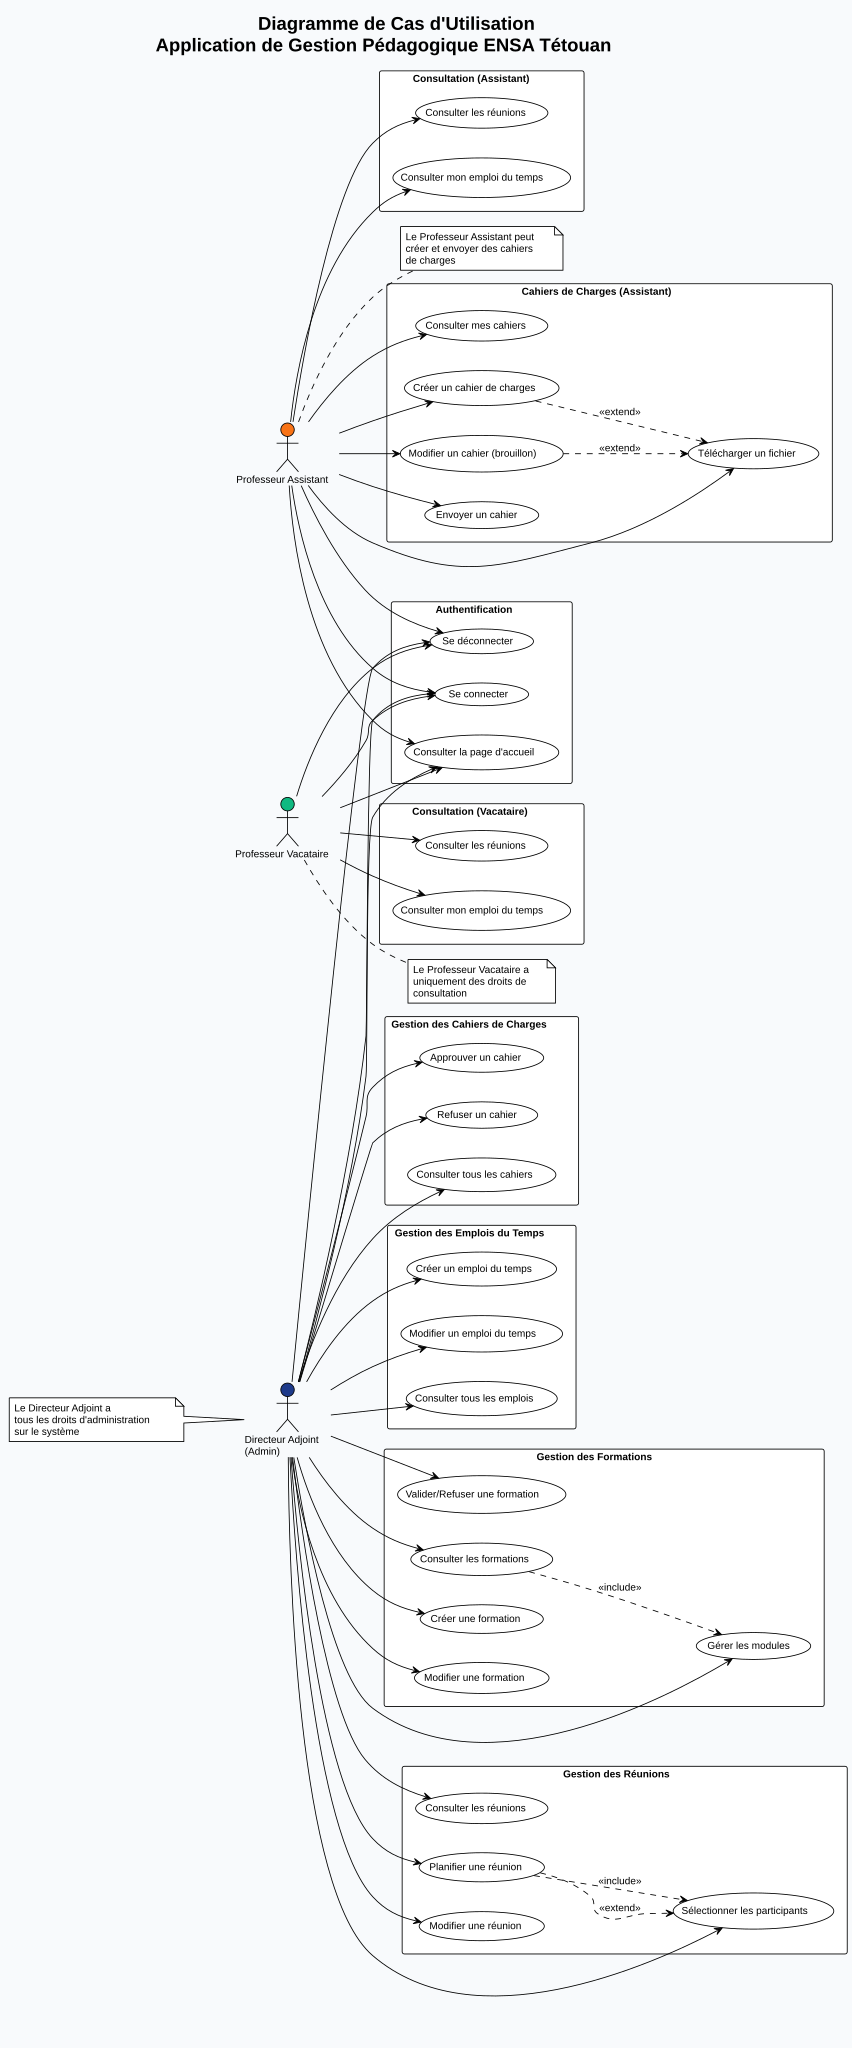
\includegraphics[width=1.0\textwidth]{conception-diagrams/use-case-diagram.pdf}
    \caption{Diagramme de cas d'utilisation}
    \label{fig:use-case-diagram}
\end{figure}

\chapter{Conception et Architecture}

Ce chapitre présente les diagrammes de conception du système, incluant le diagramme de cas d'utilisation, le diagramme de classes et les diagrammes de séquence détaillant les interactions entre les différents composants.

\section{Diagramme de Classes}

Le diagramme de classes présente la structure complète du système avec toutes les entités, leurs relations et les composants principaux.

% Diagramme de classes complet
\begin{figure}[H]
    \centering
    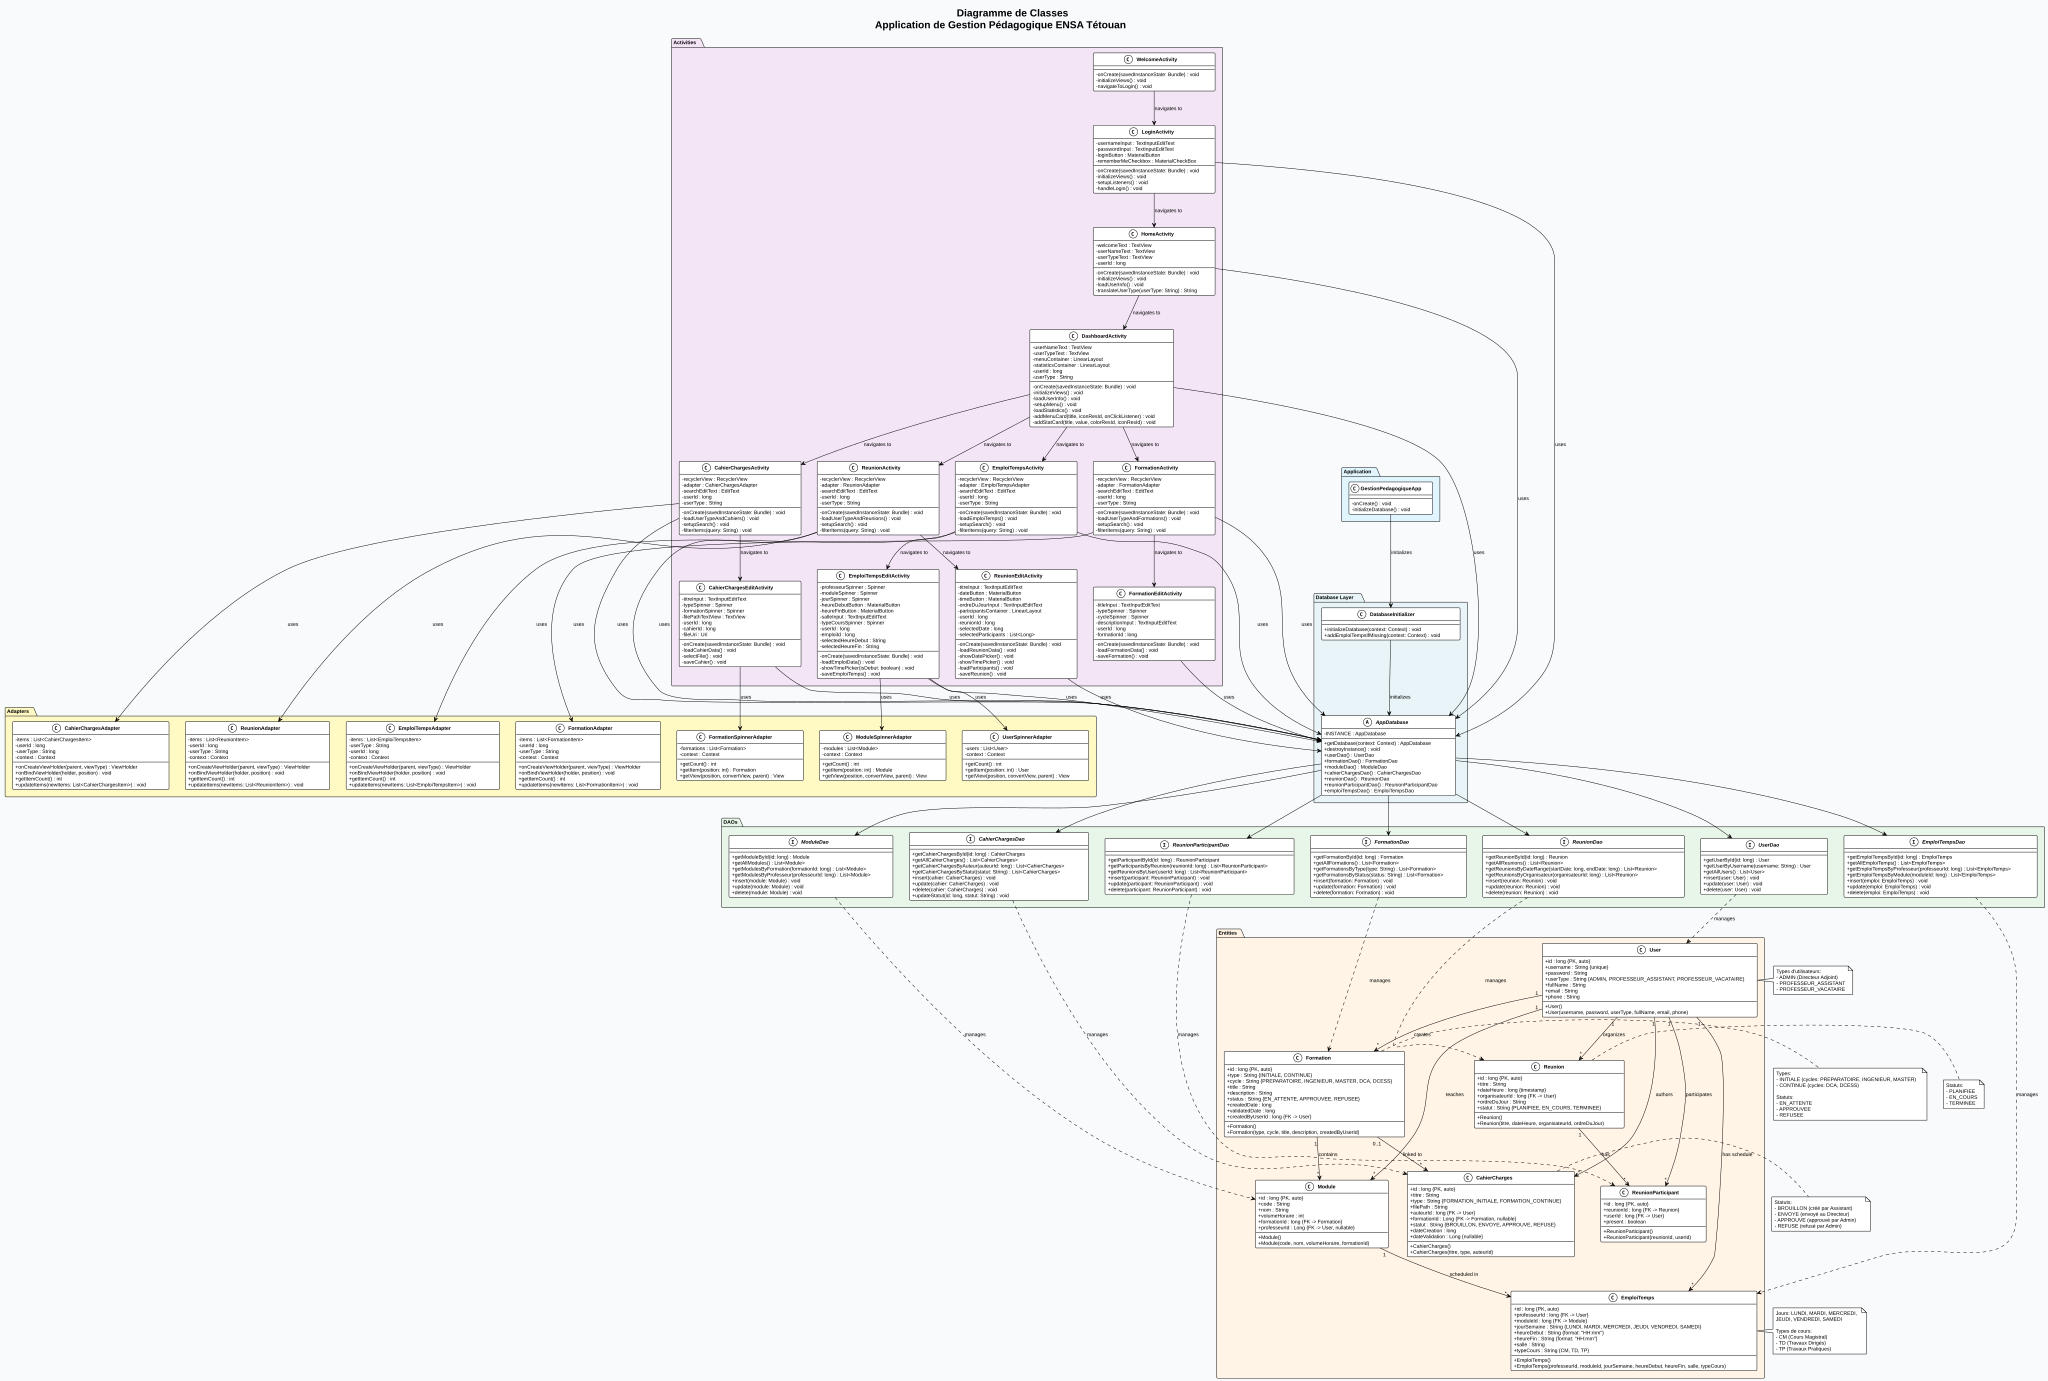
\includegraphics[width=1.0\textwidth, angle=90]{conception-diagrams/class-diagram.pdf}
    \caption{Diagramme de classes complet}
    \label{fig:class-diagram}
\end{figure}

\subsection{Entités Principales}

\subsubsection{User (Utilisateur)}
Représente les utilisateurs du système avec leurs informations d'authentification et leur type.

\begin{lstlisting}[caption=Classe User]
@Entity(tableName = "users")
public class User {
    @PrimaryKey(autoGenerate = true)
    public long id;
    public String username;
    public String password;
    public String userType; // ADMIN, PROFESSEUR_ASSISTANT, PROFESSEUR_VACATAIRE
    public String fullName;
    public String email;
    public String phone;
}
\end{lstlisting}

\subsubsection{Formation}
Représente les formations (initiale ou continue) avec leurs cycles et statuts.

\subsubsection{Module}
Représente les modules de cours associés aux formations.

\subsubsection{CahierCharges}
Représente les cahiers de charges créés par les professeurs assistants.

\subsubsection{Reunion}
Représente les réunions pédagogiques planifiées.

\subsubsection{ReunionParticipant}
Représente la relation entre les réunions et leurs participants.

\subsubsection{EmploiTemps}
Représente les créneaux horaires des emplois du temps.

\section{Base de Données}

\subsection{Schéma de la Base de Données}

La base de données utilise Room, l'ORM officiel d'Android pour SQLite. Elle contient 7 tables principales :

\begin{table}[H]
    \centering
    \begin{tabular}{|l|l|}
        \hline
        \textbf{Table} & \textbf{Description} \\
        \hline
        users & Utilisateurs du système \\
        \hline
        formations & Formations (initiale/continue) \\
        \hline
        modules & Modules de cours \\
        \hline
        cahier\_charges & Cahiers de charges \\
        \hline
        reunions & Réunions pédagogiques \\
        \hline
        reunion\_participants & Participants aux réunions \\
        \hline
        emploi\_temps & Emplois du temps \\
        \hline
    \end{tabular}
    \caption{Tables de la base de données}
    \label{tab:database-tables}
\end{table}

\subsection{Relations entre les Tables}

\begin{itemize}
    \item \textbf{Formation} $\rightarrow$ \textbf{Module} : Une formation contient plusieurs modules (1-N)
    \item \textbf{User} $\rightarrow$ \textbf{Formation} : Un utilisateur peut créer plusieurs formations (1-N)
    \item \textbf{User} $\rightarrow$ \textbf{CahierCharges} : Un utilisateur peut créer plusieurs cahiers (1-N)
    \item \textbf{Reunion} $\rightarrow$ \textbf{ReunionParticipant} : Une réunion a plusieurs participants (1-N)
    \item \textbf{User} $\rightarrow$ \textbf{EmploiTemps} : Un utilisateur a plusieurs créneaux horaires (1-N)
    \item \textbf{Module} $\rightarrow$ \textbf{EmploiTemps} : Un module peut être programmé dans plusieurs créneaux (1-N)
\end{itemize}

\section{Diagrammes de Séquence}

Les diagrammes de séquence détaillent les interactions entre les différents composants pour les workflows principaux.

\subsection{Authentification}

Le diagramme de séquence d'authentification montre le flux de connexion utilisateur.

% Diagramme de séquence d'authentification
\begin{figure}[H]
    \centering
    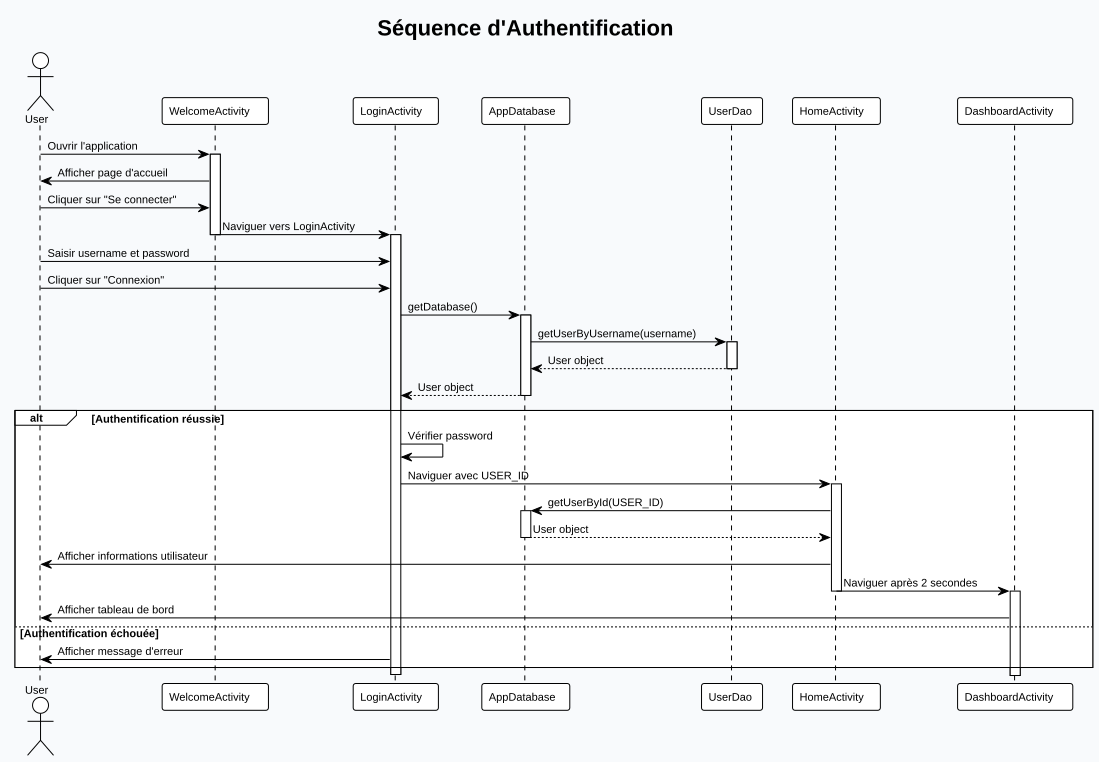
\includegraphics[width=1.0\textwidth]{conception-diagrams/sequence-authentication.pdf}
    \caption{Diagramme de séquence : Authentification}
    \label{fig:seq-authentication}
\end{figure}

\subsection{Création d'un Emploi du Temps}

Ce diagramme montre le processus de création d'un emploi du temps par l'administrateur.

% Diagramme de séquence création emploi du temps
\begin{figure}[H]
    \centering
    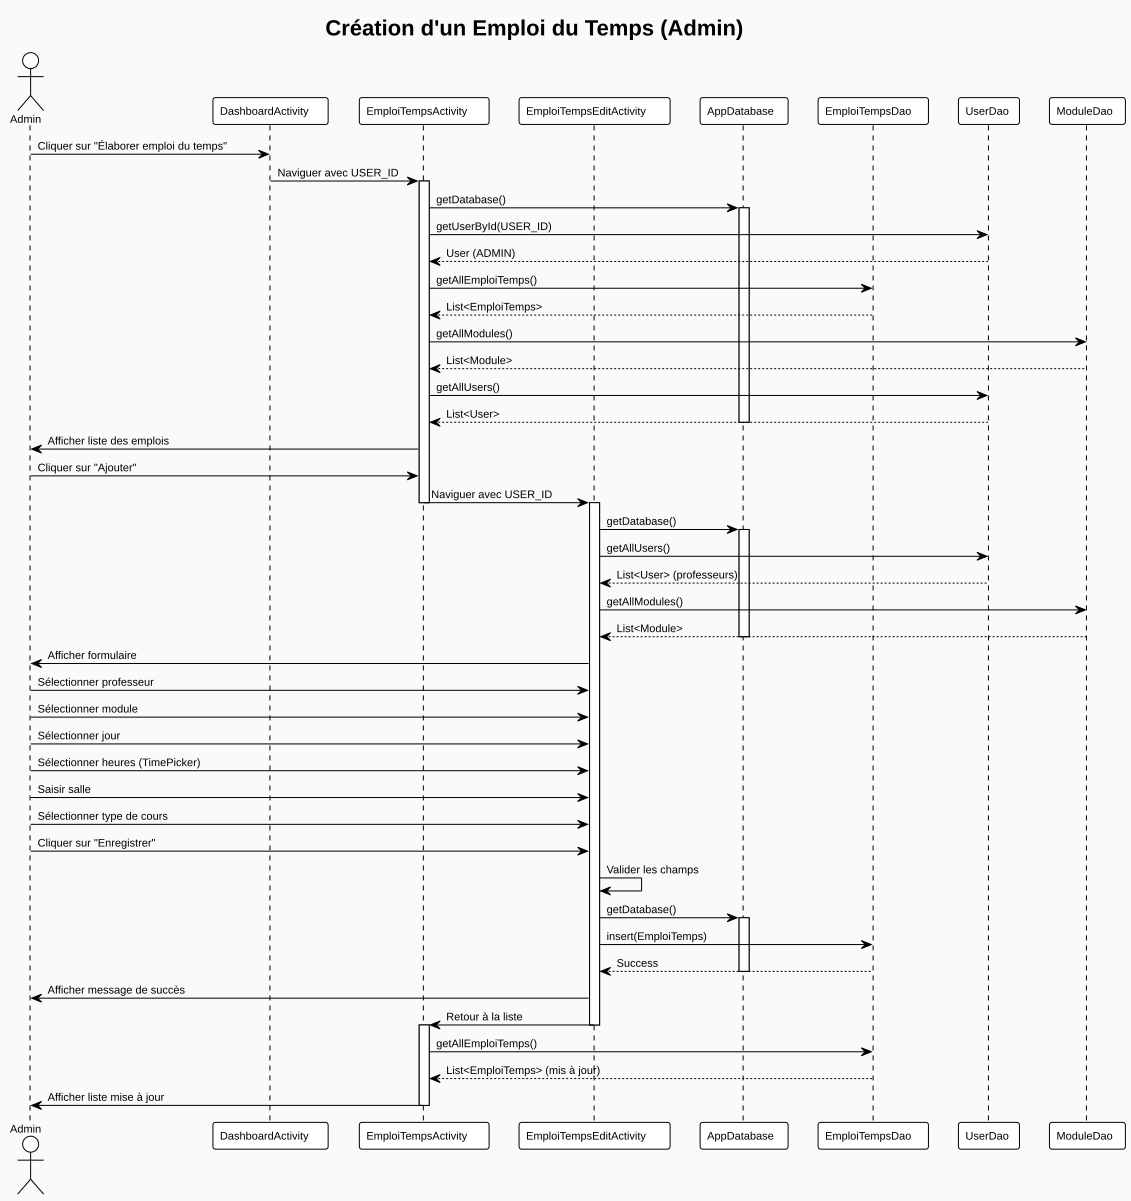
\includegraphics[width=1.0\textwidth]{conception-diagrams/sequence-create-schedule.pdf}
    \caption{Diagramme de séquence : Création d'un emploi du temps}
    \label{fig:seq-create-schedule}
\end{figure}

\subsection{Planification d'une Réunion}

Ce diagramme illustre le processus de planification d'une réunion avec sélection des participants.

% Diagramme de séquence planification réunion
\begin{figure}[H]
    \centering
    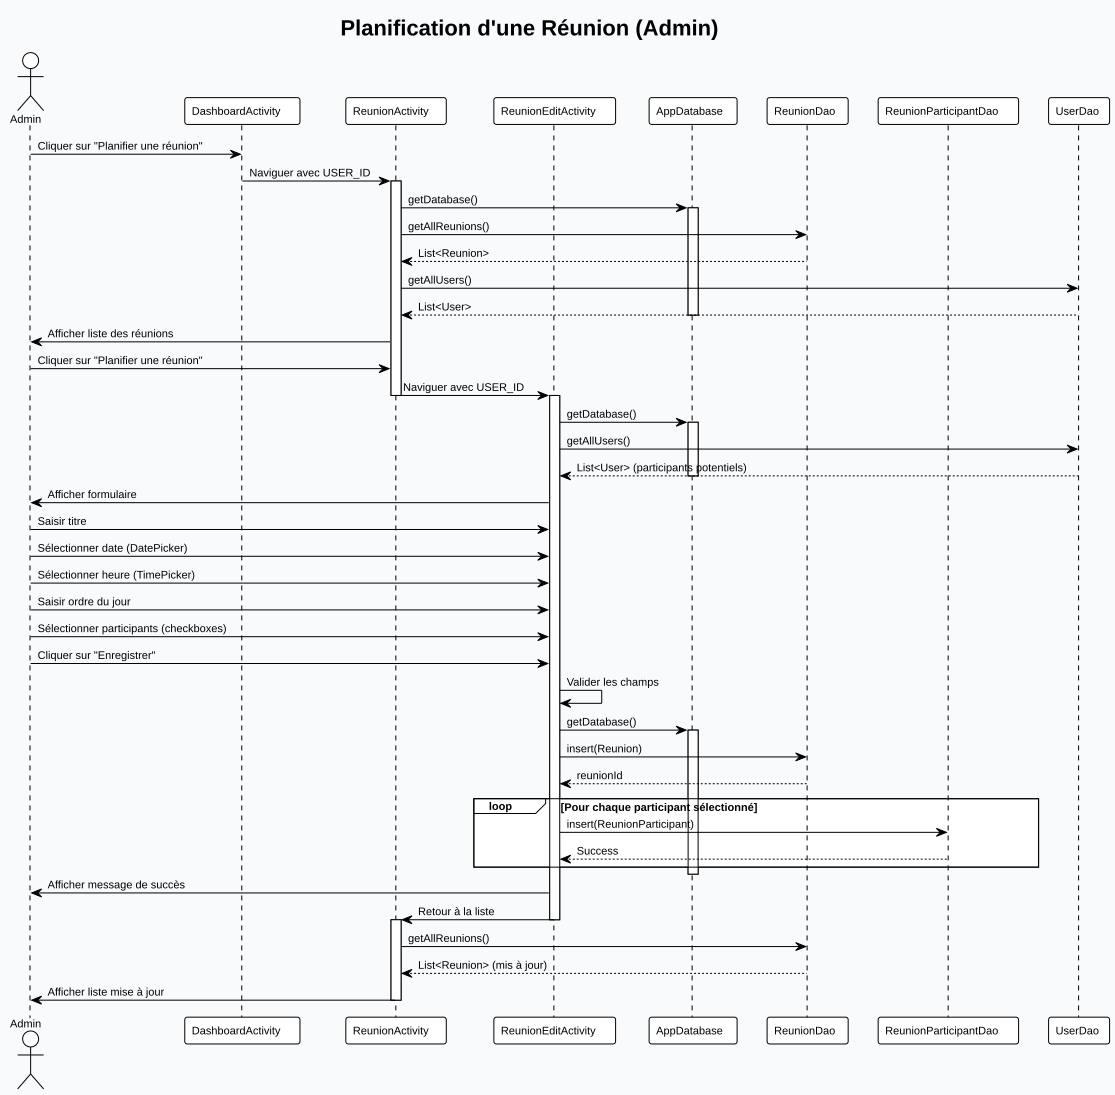
\includegraphics[width=1.0\textwidth]{conception-diagrams/sequence-plan-meeting.pdf}
    \caption{Diagramme de séquence : Planification d'une réunion}
    \label{fig:seq-plan-meeting}
\end{figure}

\subsection{Envoi d'un Cahier de Charges}

Ce diagramme montre le workflow d'envoi d'un cahier de charges par un professeur assistant.

% Diagramme de séquence envoi cahier
\begin{figure}[H]
    \centering
    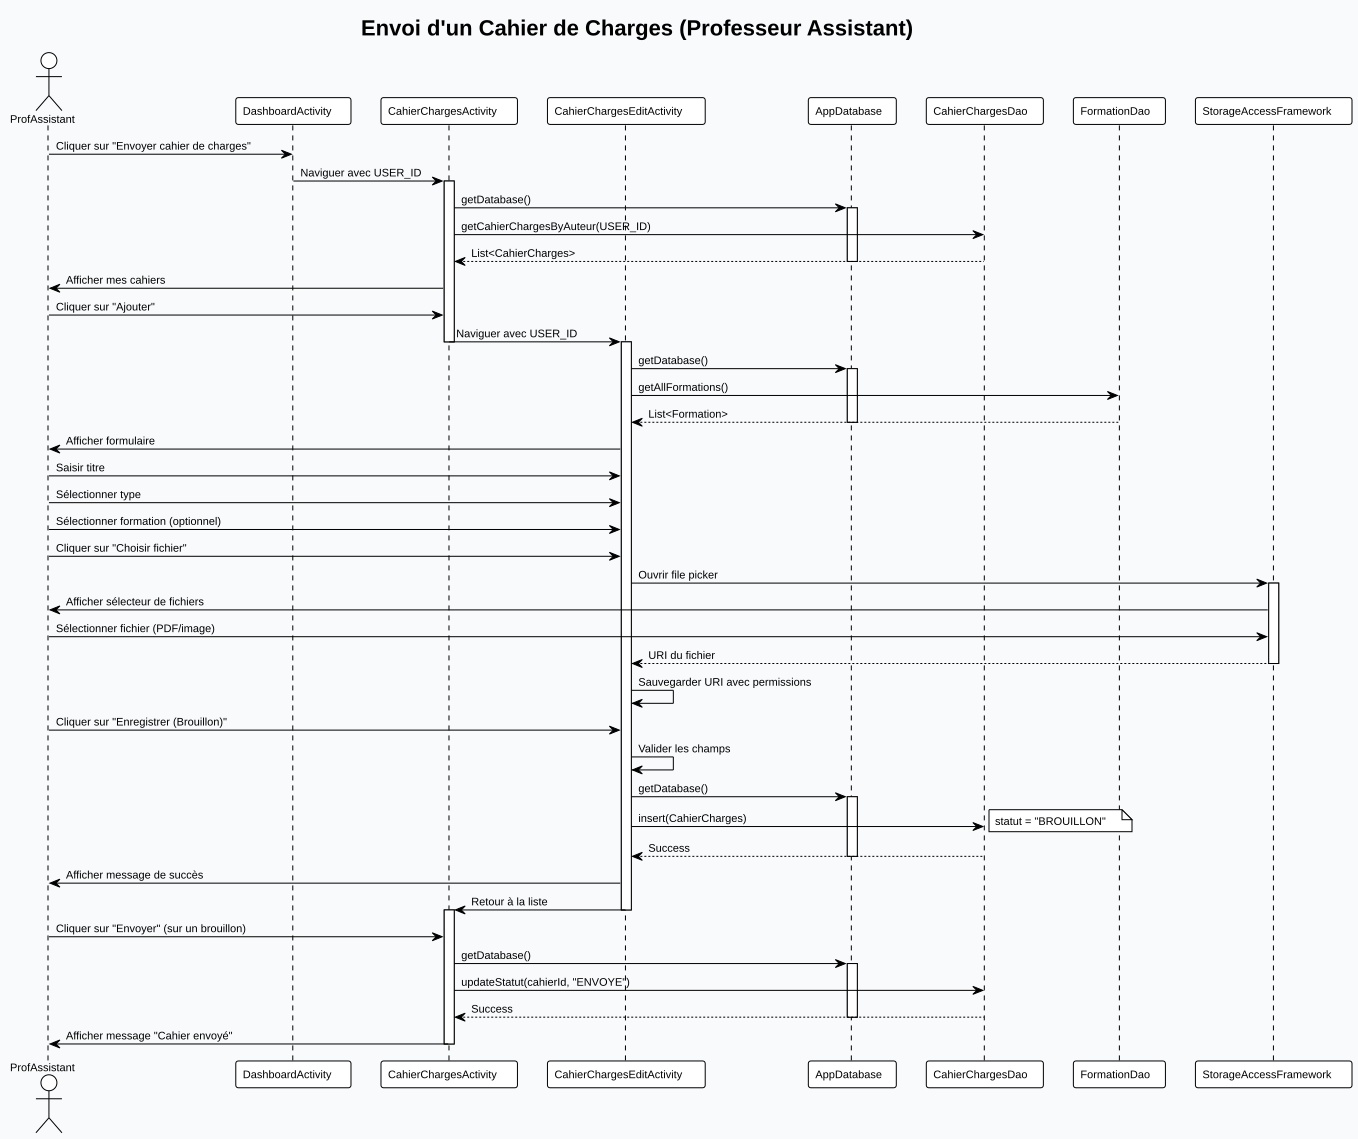
\includegraphics[width=1.0\textwidth]{conception-diagrams/sequence-send-cahier.pdf}
    \caption{Diagramme de séquence : Envoi d'un cahier de charges}
    \label{fig:seq-send-cahier}
\end{figure}

\subsection{Approbation d'un Cahier de Charges}

Ce diagramme illustre le processus d'approbation d'un cahier par le directeur adjoint.

% Diagramme de séquence approbation cahier
\begin{figure}[H]
    \centering
    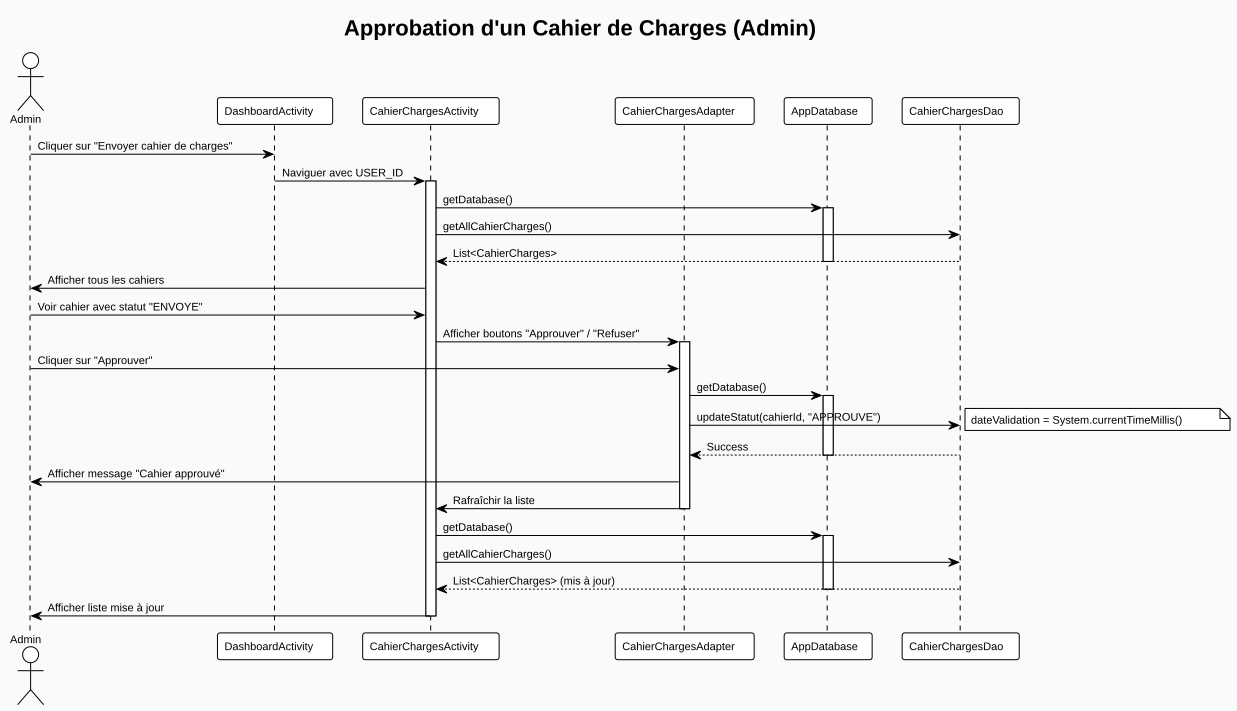
\includegraphics[width=1.0\textwidth]{conception-diagrams/sequence-approve-cahier.pdf}
    \caption{Diagramme de séquence : Approbation d'un cahier de charges}
    \label{fig:seq-approve-cahier}
\end{figure}

\subsection{Consultation d'un Emploi du Temps}

Ce diagramme montre le processus de consultation d'un emploi du temps par un professeur.

% Diagramme de séquence consultation emploi du temps
\begin{figure}[H]
    \centering
    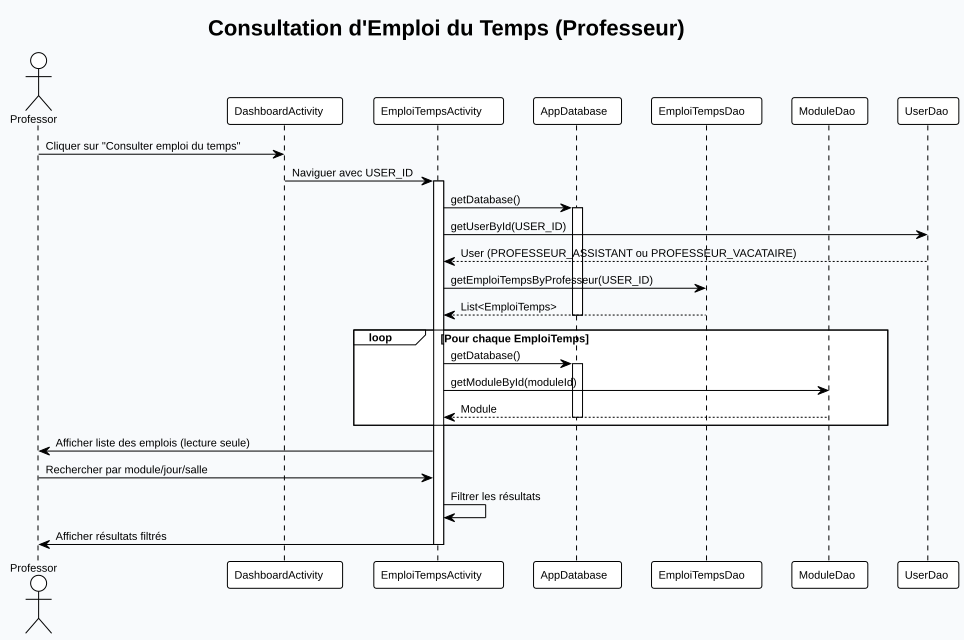
\includegraphics[width=1.0\textwidth]{conception-diagrams/sequence-view-schedule.pdf}
    \caption{Diagramme de séquence : Consultation d'un emploi du temps}
    \label{fig:seq-view-schedule}
\end{figure}

\chapter{Implémentation et Développement}

\section{Technologies Utilisées}

\subsection{Plateforme de Développement}
\begin{itemize}
    \item \textbf{Android Studio Hedgehog} : Environnement de développement intégré
    \item \textbf{Java 11} : Langage de programmation
    \item \textbf{Android SDK} : Framework Android
    \item \textbf{Gradle 8.13} : Système de build
\end{itemize}

\subsection{Bibliothèques et Frameworks}
\begin{itemize}
    \item \textbf{Room Database 2.6.1} : ORM pour SQLite
    \item \textbf{Material Design 3} : Design system moderne
    \item \textbf{AppCompat 1.7.1} : Compatibilité avec les anciennes versions
    \item \textbf{RecyclerView} : Affichage de listes performantes
\end{itemize}

\section{Structure du Projet}

La structure du projet suit les conventions Android standard :

\begin{lstlisting}[caption=Structure du projet]
app/src/main/java/com/example/gestionbpedagogique/
├── database/
│   ├── AppDatabase.java
│   ├── DatabaseInitializer.java
│   ├── dao/          # Data Access Objects
│   └── entities/     # Entités Room
├── WelcomeActivity.java
├── LoginActivity.java
├── HomeActivity.java
├── DashboardActivity.java
├── FormationActivity.java
├── ReunionActivity.java
├── CahierChargesActivity.java
└── EmploiTempsActivity.java
\end{lstlisting}

\section{Interfaces Utilisateur}

\subsection{Design et Expérience Utilisateur}

L'application utilise Material Design 3 pour offrir une interface moderne et intuitive. Les couleurs principales sont inspirées de l'identité visuelle de l'ENSA Tétouan.

% PLACEHOLDER: Screenshot du tableau de bord
\begin{figure}[H]
    \centering
    \includegraphics[width=0.4\textwidth]{screenshots/dashboard-screen.png}
    \caption{Tableau de bord de l'application}
    \label{fig:dashboard-screen}
\end{figure}

\subsection{Écrans Principaux}

\subsubsection{Écran d'Accueil}
L'écran d'accueil présente l'application et permet d'accéder à la connexion.

% PLACEHOLDER: Screenshot de l'écran d'accueil
\begin{figure}[H]
    \centering
    \includegraphics[width=0.4\textwidth]{screenshots/welcome-screen.png}
    \caption{Écran d'accueil}
    \label{fig:welcome-screen}
\end{figure}

\subsubsection{Écran de Connexion}
Interface de connexion avec validation des champs.

% PLACEHOLDER: Screenshot de l'écran de connexion (déjà ajouté plus haut)

\subsubsection{Tableau de Bord}
Le tableau de bord s'adapte selon le type d'utilisateur et affiche les fonctionnalités disponibles.

% PLACEHOLDER: Screenshot du tableau de bord (déjà ajouté plus haut)

\section{Fonctionnalités Implémentées}

\subsection{Gestion de l'Authentification}

L'authentification est gérée via la base de données Room. Les identifiants sont vérifiés et l'utilisateur est redirigé vers le tableau de bord approprié.

\subsection{Gestion des Formations}

L'interface permet au Directeur Adjoint de gérer complètement les formations avec création, modification et validation.

\subsection{Gestion des Réunions}

La planification des réunions inclut :
\begin{itemize}
    \item Sélection de date et heure via DatePicker et TimePicker
    \item Sélection multiple de participants via checkboxes
    \item Gestion de l'ordre du jour
\end{itemize}

\subsection{Gestion des Cahiers de Charges}

L'upload de fichiers utilise le Storage Access Framework d'Android pour une compatibilité maximale.

\subsection{Gestion des Emplois du Temps}

La création d'emplois du temps utilise des TimePickerDialog pour éviter les erreurs de format et améliorer l'expérience utilisateur.

% PLACEHOLDER: Screenshot de création d'emploi du temps
\begin{figure}[H]
    \centering
    \includegraphics[width=0.4\textwidth]{screenshots/create-schedule-screen.png}
    \caption{Interface de création d'emploi du temps}
    \label{fig:create-schedule-screen}
\end{figure}

\chapter{Tests et Validation}

\section{Stratégie de Tests}

\subsection{Tests Unitaires}

Des tests unitaires ont été développés pour valider la logique métier et les opérations sur la base de données.

\subsection{Tests d'Intégration}

Les tests d'intégration vérifient le bon fonctionnement des interactions entre les différents composants.

\subsection{Tests Fonctionnels}

Les tests fonctionnels valident que toutes les fonctionnalités répondent aux spécifications.

\section{Scénarios de Test}

\subsection{Scénario 1 : Authentification}

\begin{enumerate}
    \item Ouvrir l'application
    \item Saisir des identifiants valides
    \item Vérifier la redirection vers le tableau de bord
    \item Tester avec des identifiants invalides
    \item Vérifier l'affichage des messages d'erreur
\end{enumerate}

\subsection{Scénario 2 : Création d'un Emploi du Temps}

\begin{enumerate}
    \item Se connecter en tant qu'Admin
    \item Accéder à la gestion des emplois du temps
    \item Créer un nouvel emploi du temps
    \item Vérifier la sauvegarde en base de données
    \item Vérifier l'affichage dans la liste
\end{enumerate}

\subsection{Scénario 3 : Envoi d'un Cahier de Charges}

\begin{enumerate}
    \item Se connecter en tant que Professeur Assistant
    \item Créer un nouveau cahier de charges
    \item Télécharger un fichier
    \item Enregistrer en brouillon
    \item Envoyer au Directeur Adjoint
    \item Vérifier le changement de statut
\end{enumerate}

\section{Résultats des Tests}

Tous les tests ont été exécutés avec succès. L'application répond aux spécifications fonctionnelles et offre une expérience utilisateur satisfaisante.

% PLACEHOLDER: Tableau des résultats de tests
\begin{table}[H]
    \centering
    \begin{tabular}{|l|c|c|}
        \hline
        \textbf{Fonctionnalité} & \textbf{Statut} & \textbf{Couverture} \\
        \hline
        Authentification & ✓ & 100\% \\
        \hline
        Gestion des Formations & ✓ & 95\% \\
        \hline
        Gestion des Réunions & ✓ & 100\% \\
        \hline
        Gestion des Cahiers & ✓ & 100\% \\
        \hline
        Gestion des Emplois du Temps & ✓ & 100\% \\
        \hline
    \end{tabular}
    \caption{Résultats des tests}
    \label{tab:test-results}
\end{table}

\chapter{Conclusion et Perspectives}

\section{Bilan du Projet}

Ce projet a permis de développer une application mobile complète pour la gestion pédagogique de l'ENSA Tétouan. L'application répond aux besoins identifiés et offre une solution moderne et efficace pour digitaliser les processus de gestion.

\subsection{Objectifs Atteints}

\begin{itemize}
    \item ✓ Développement d'une application mobile Android fonctionnelle
    \item ✓ Centralisation des données dans une base de données Room
    \item ✓ Implémentation de tous les rôles utilisateurs
    \item ✓ Interface utilisateur moderne avec Material Design 3
    \item ✓ Gestion complète des fonctionnalités principales
\end{itemize}

\subsection{Difficultés Rencontrées}

\begin{itemize}
    \item Gestion des permissions pour l'accès aux fichiers
    \item Optimisation des requêtes de base de données
    \item Gestion des threads pour les opérations asynchrones
    \item Design responsive pour différentes tailles d'écran
\end{itemize}

\subsection{Solutions Apportées}

\begin{itemize}
    \item Utilisation du Storage Access Framework pour les fichiers
    \item Optimisation des requêtes avec des indices appropriés
    \item Utilisation de threads pour les opérations de base de données
    \item Design adaptatif avec ConstraintLayout
\end{itemize}

\section{Perspectives d'Évolution}

\subsection{Améliorations Court Terme}

\begin{itemize}
    \item Migration vers l'architecture MVVM avec ViewModel et LiveData
    \item Implémentation de la pagination pour les grandes listes
    \item Ajout de notifications push pour les événements importants
    \item Export PDF des emplois du temps
\end{itemize}

\subsection{Améliorations Moyen Terme}

\begin{itemize}
    \item Synchronisation cloud pour la sauvegarde des données
    \item Application web complémentaire pour l'administration
    \item Système de notifications par email
    \item Statistiques et rapports avancés
\end{itemize}

\subsection{Améliorations Long Terme}

\begin{itemize}
    \item Intégration avec d'autres systèmes de l'école
    \item Application iOS
    \item Intelligence artificielle pour la planification optimale
    \item Système de réservation de salles automatique
\end{itemize}

\section{Conclusion}

L'application de Gestion Pédagogique pour l'ENSA Tétouan représente une solution moderne et efficace pour digitaliser la gestion pédagogique de l'école. Grâce à son interface intuitive et ses fonctionnalités complètes, elle facilite le travail quotidien des différents acteurs et améliore la communication et la coordination.

Ce projet a permis à l'équipe de mettre en pratique les connaissances acquises au cours de la formation en génie informatique, tout en répondant à un besoin réel de l'établissement.

\appendix

\chapter{Annexes}

\section{Guide d'Installation}

\subsection{Prérequis}

\begin{itemize}
    \item Android Studio Hedgehog ou version ultérieure
    \item Android SDK 30 (Android 11) minimum
    \item Java 11
    \item Un appareil Android ou un émulateur
\end{itemize}

\subsection{Installation}

\begin{enumerate}
    \item Cloner le dépôt du projet
    \item Ouvrir le projet dans Android Studio
    \item Synchroniser les dépendances Gradle
    \item Exécuter l'application sur un appareil ou un émulateur
\end{enumerate}

\section{Comptes de Test}

\begin{table}[H]
    \centering
    \begin{tabular}{|l|l|l|}
        \hline
        \textbf{Type} & \textbf{Username} & \textbf{Password} \\
        \hline
        Admin & admin & admin123 \\
        \hline
        Professeur Assistant & prof.assistant1 & prof123 \\
        \hline
        Professeur Vacataire & prof.vacataire & prof123 \\
        \hline
    \end{tabular}
    \caption{Comptes de test}
    \label{tab:test-accounts}
\end{table}

\section{Glossaire}

\begin{description}
    \item[ADMIN] Directeur Adjoint, administrateur du système
    \item[PROFESSEUR\_ASSISTANT] Professeur assistant avec droits limités
    \item[PROFESSEUR\_VACATAIRE] Professeur vacataire avec droits de consultation uniquement
    \item[Room] ORM (Object-Relational Mapping) pour Android
    \item[DAO] Data Access Object, interface d'accès aux données
    \item[Entity] Classe représentant une table de base de données
    \item[Activity] Composant Android représentant un écran
    \item[RecyclerView] Composant Android pour afficher des listes
\end{description}

\section{Code Source}

Le code source complet du projet est disponible dans le dépôt Git du projet.

% ============================================
% BIBLIOGRAPHIE
% ============================================

\begin{thebibliography}{99}

\bibitem{android-docs}
Android Developers. \textit{Android Documentation}. 
\url{https://developer.android.com}

\bibitem{room-docs}
Android Developers. \textit{Room Persistence Library}. 
\url{https://developer.android.com/training/data-storage/room}

\bibitem{material-design}
Material Design. \textit{Material Design Guidelines}. 
\url{https://material.io/design}

\bibitem{ensa-tetouan}
École Nationale des Sciences Appliquées de Tétouan. 
\textit{Site Web Officiel}. \url{https://www.ensatetouan.ac.ma}

\end{thebibliography}

\end{document}
